\section{Energetic particles in the heliosphere}
\label{sec:particles_heliosphere}
\begin{figure}
	\centering
	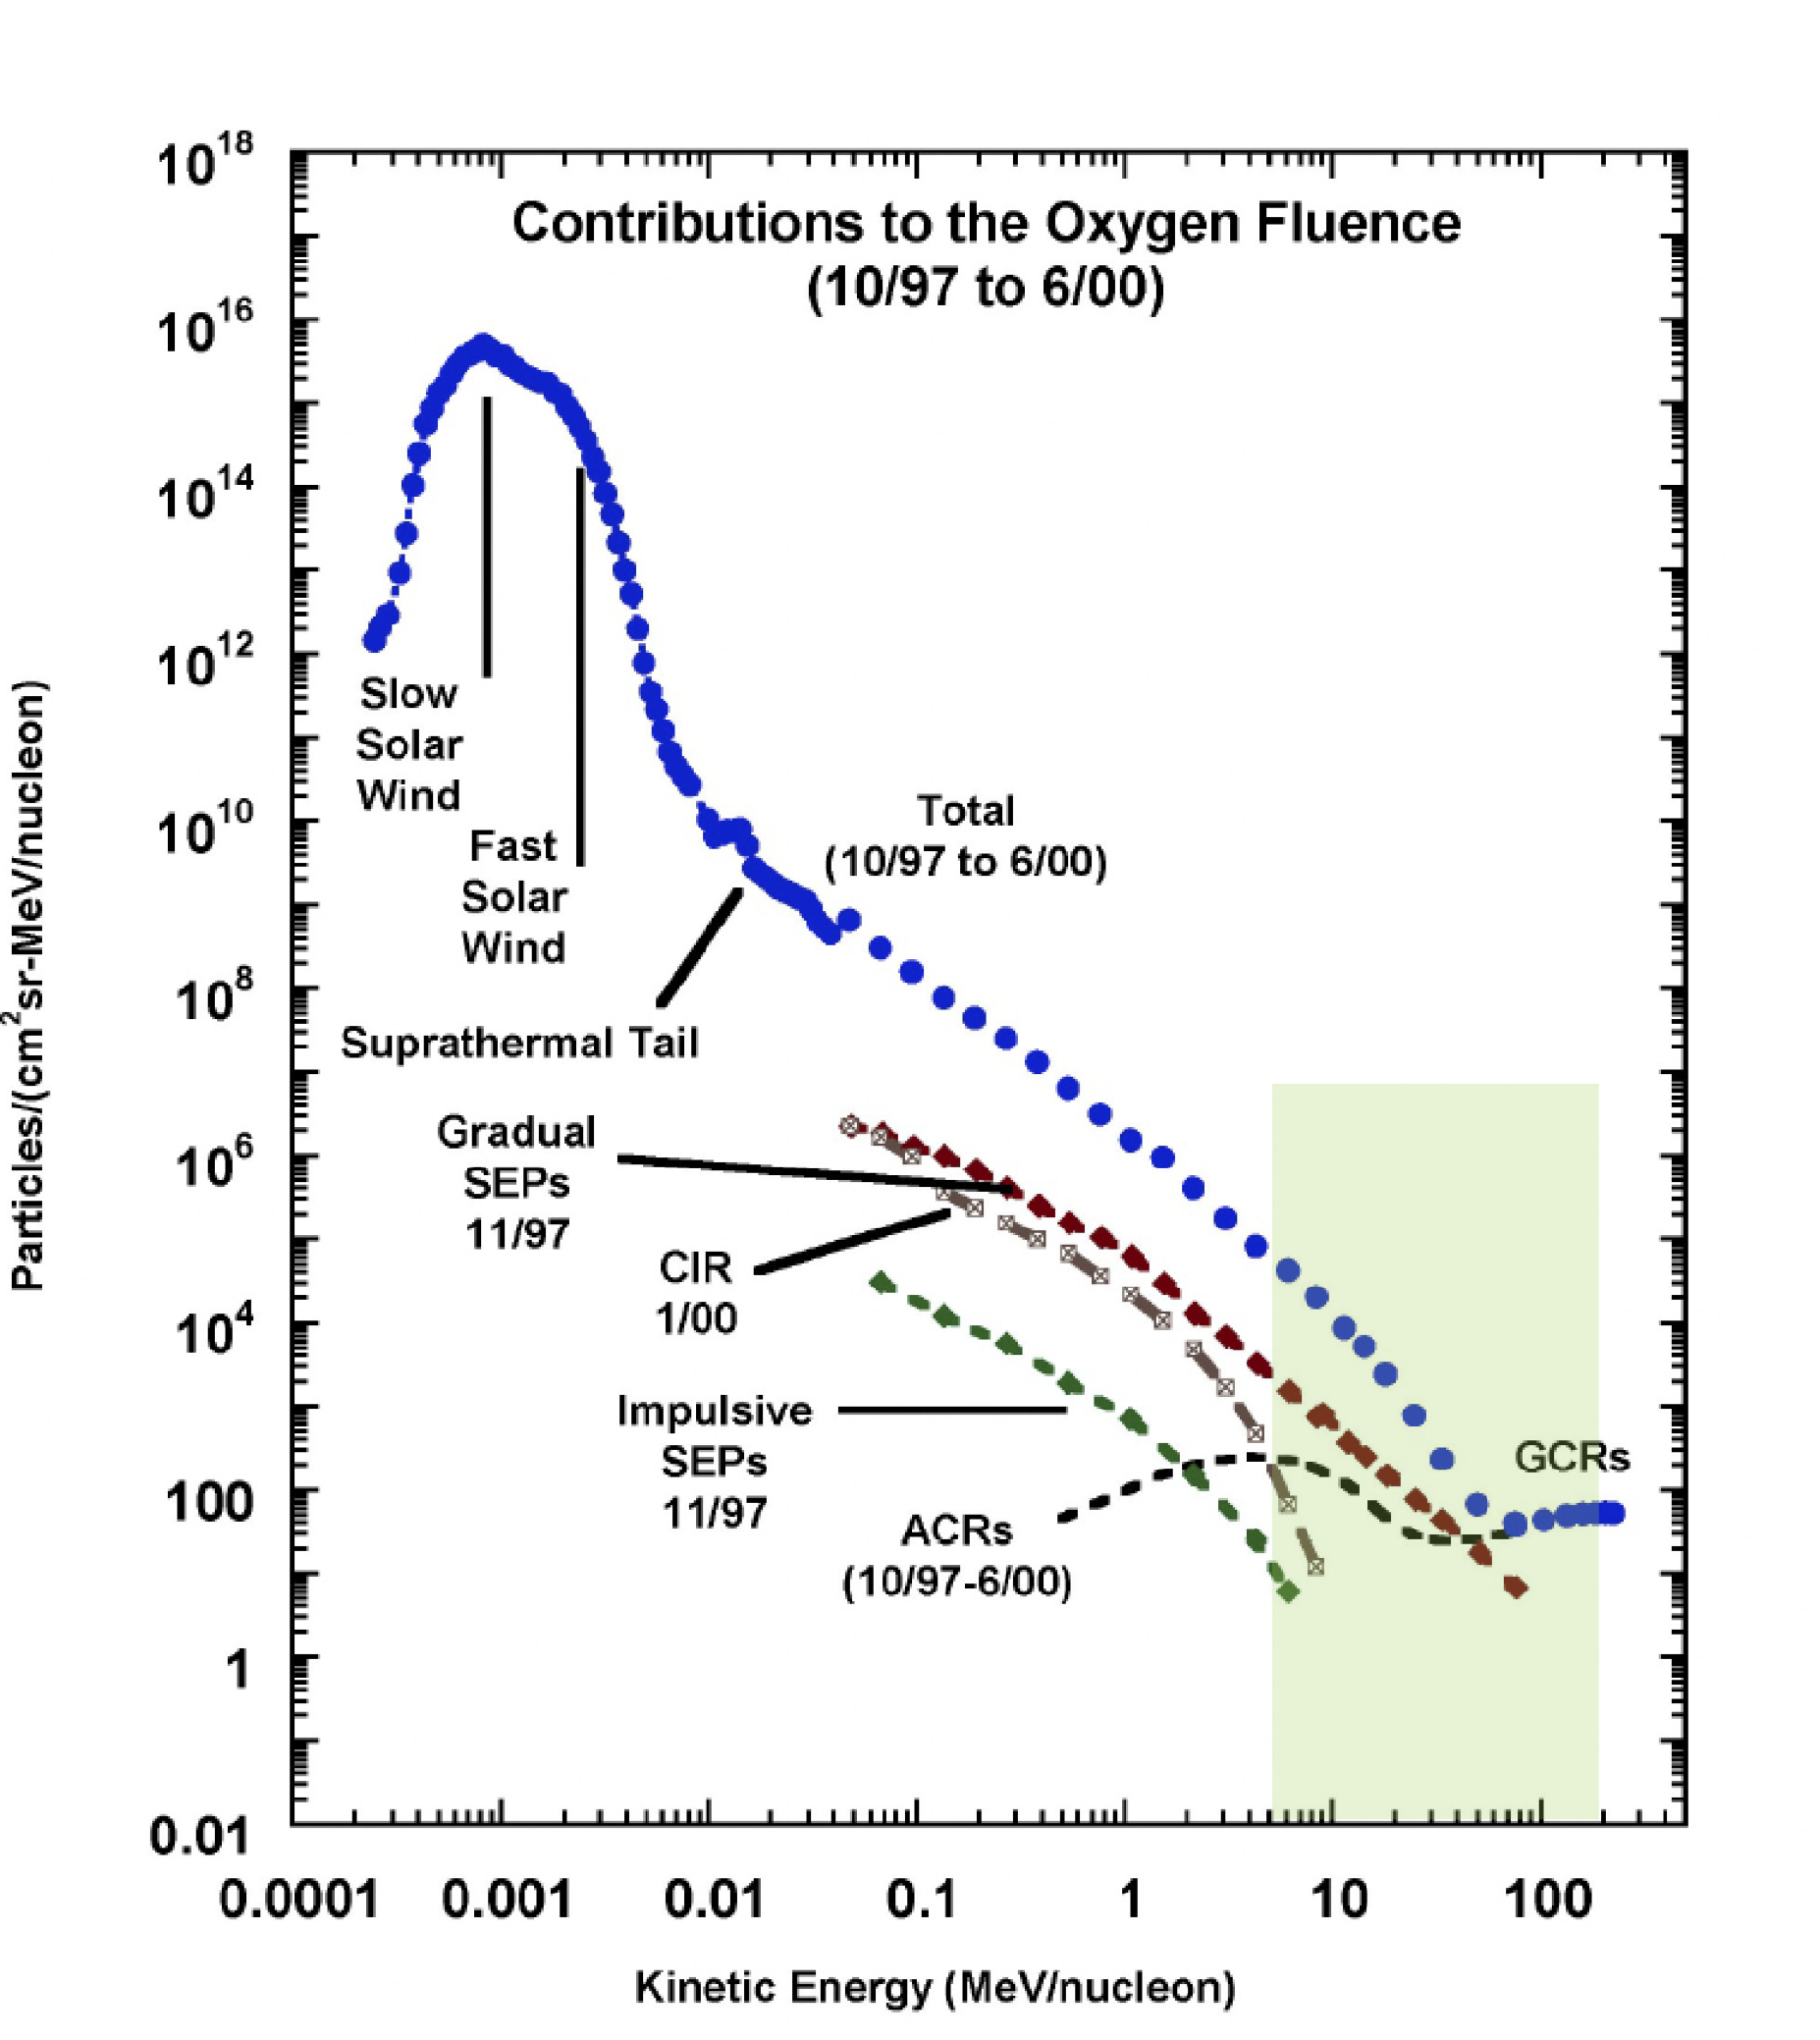
\includegraphics[width = 0.6\textwidth]{images/heliospheric_particle_spectra_color.png}
	\caption[Energy spectra of oxygen ions in the near Earth space]{The typical oxygen spectra in the interplanetary space near the Earth, indicating the contributions of different populations, especially in the energy range between few MeV\/nuc and few hundreds MeV\/nuc, where \acs{SEP}, \acs{ACR} and \acs{GCR} both exist. The spectra of other particles species for instance, helium and proton, have the similar shape but different flux level on corresponding energy region. The figure is adapted from \cite{Mewaldt-2001}}
	\label{Fig:Oxygen_spectra_heliosphere}
\end{figure}

\begin{itemize}
	\item The few tens of MeV energy range is an very important energy range for the heliosphere. In this part the SEP, ACR, lower GCR are bothe there. Therefore, more attention required here
	\item 
\end{itemize}



\section{SEP}

discovery of SEP and history of SEP
- first SEP
- 

Two type of SEP and how the source of SEP evolved

Wide spread SEP

Multi-instrument observation of the SE
The problem of SEP studies



\section{GCR}

primary observation of GCR
	GCR source  - how the GCR generated

	GCR composite of 

GCR solar modulation

 - find a review and summarized

 GCR transportation






\subsection{ACR}

Basic observation fact of ACR
- source 

modulation and Transport of Cosmic ray - magnetic field changed with solar activities and affect the transport -  which is reason of the radial gradient change compare to the PSP 

The 
We care about the ACR radial gradient



\subsection{Radiation hazard of energetic particle and the interaction with the planet for instance Moon and Mars}

Radiation hazard of the SEP 
- Space
- on the planetary environment
Radiation from GCR and the secondary particle generated by the GCR

- GCR interaction with regolith, lunar-
	- Generation of Neutron

The exploration of space has witnessed a surge in intensity, with an increasing number of countries aspiring to venture into this domain. Noteworthy examples include NASA's initiation of the Artemis mission, which aims to return to the Moon by 2024. Similarly, China has unveiled its plans to establish a lunar base on the lunar surface by the 2030s, while the European Space Agency (ESA) has also embarked on a lunar lander mission. Most recently, a Japanese lunar lander mission was launched; however, it regrettably encountered failure.

Under these circumstances, the study of solar energetic particles (SEPs) assumes greater significance. SEPs pose a significant radiation hazard for future human exploration on the lunar surface. The most hazardous SEP events have the potential to induce radiation increases of substantial magnitude.

\subsection{Motivition}
New instrument, new data, 
Now observation point.
new solar cycle, special solar Cycle
new solar minimum, special solar minimum





Our heliosphere is a vast region in space embedded in the \ac{ISM}, which encompasses all solar system planets and extends far beyond even the Kuiper belt. 
It is filled with a thin plasma consisting of various populations of particles, many of which originate from the Sun itself. These populations can be identified in \autoref{fig:heliospheric_energy_spectrum} \citep[based on measurements by][]{Mewaldt-2001}, shown as an energy spectrum that extends over more than 7 orders of magnitude on the energy scale and about 20 orders of magnitude on the intensity scale.
\begin{figure}
    \centering
    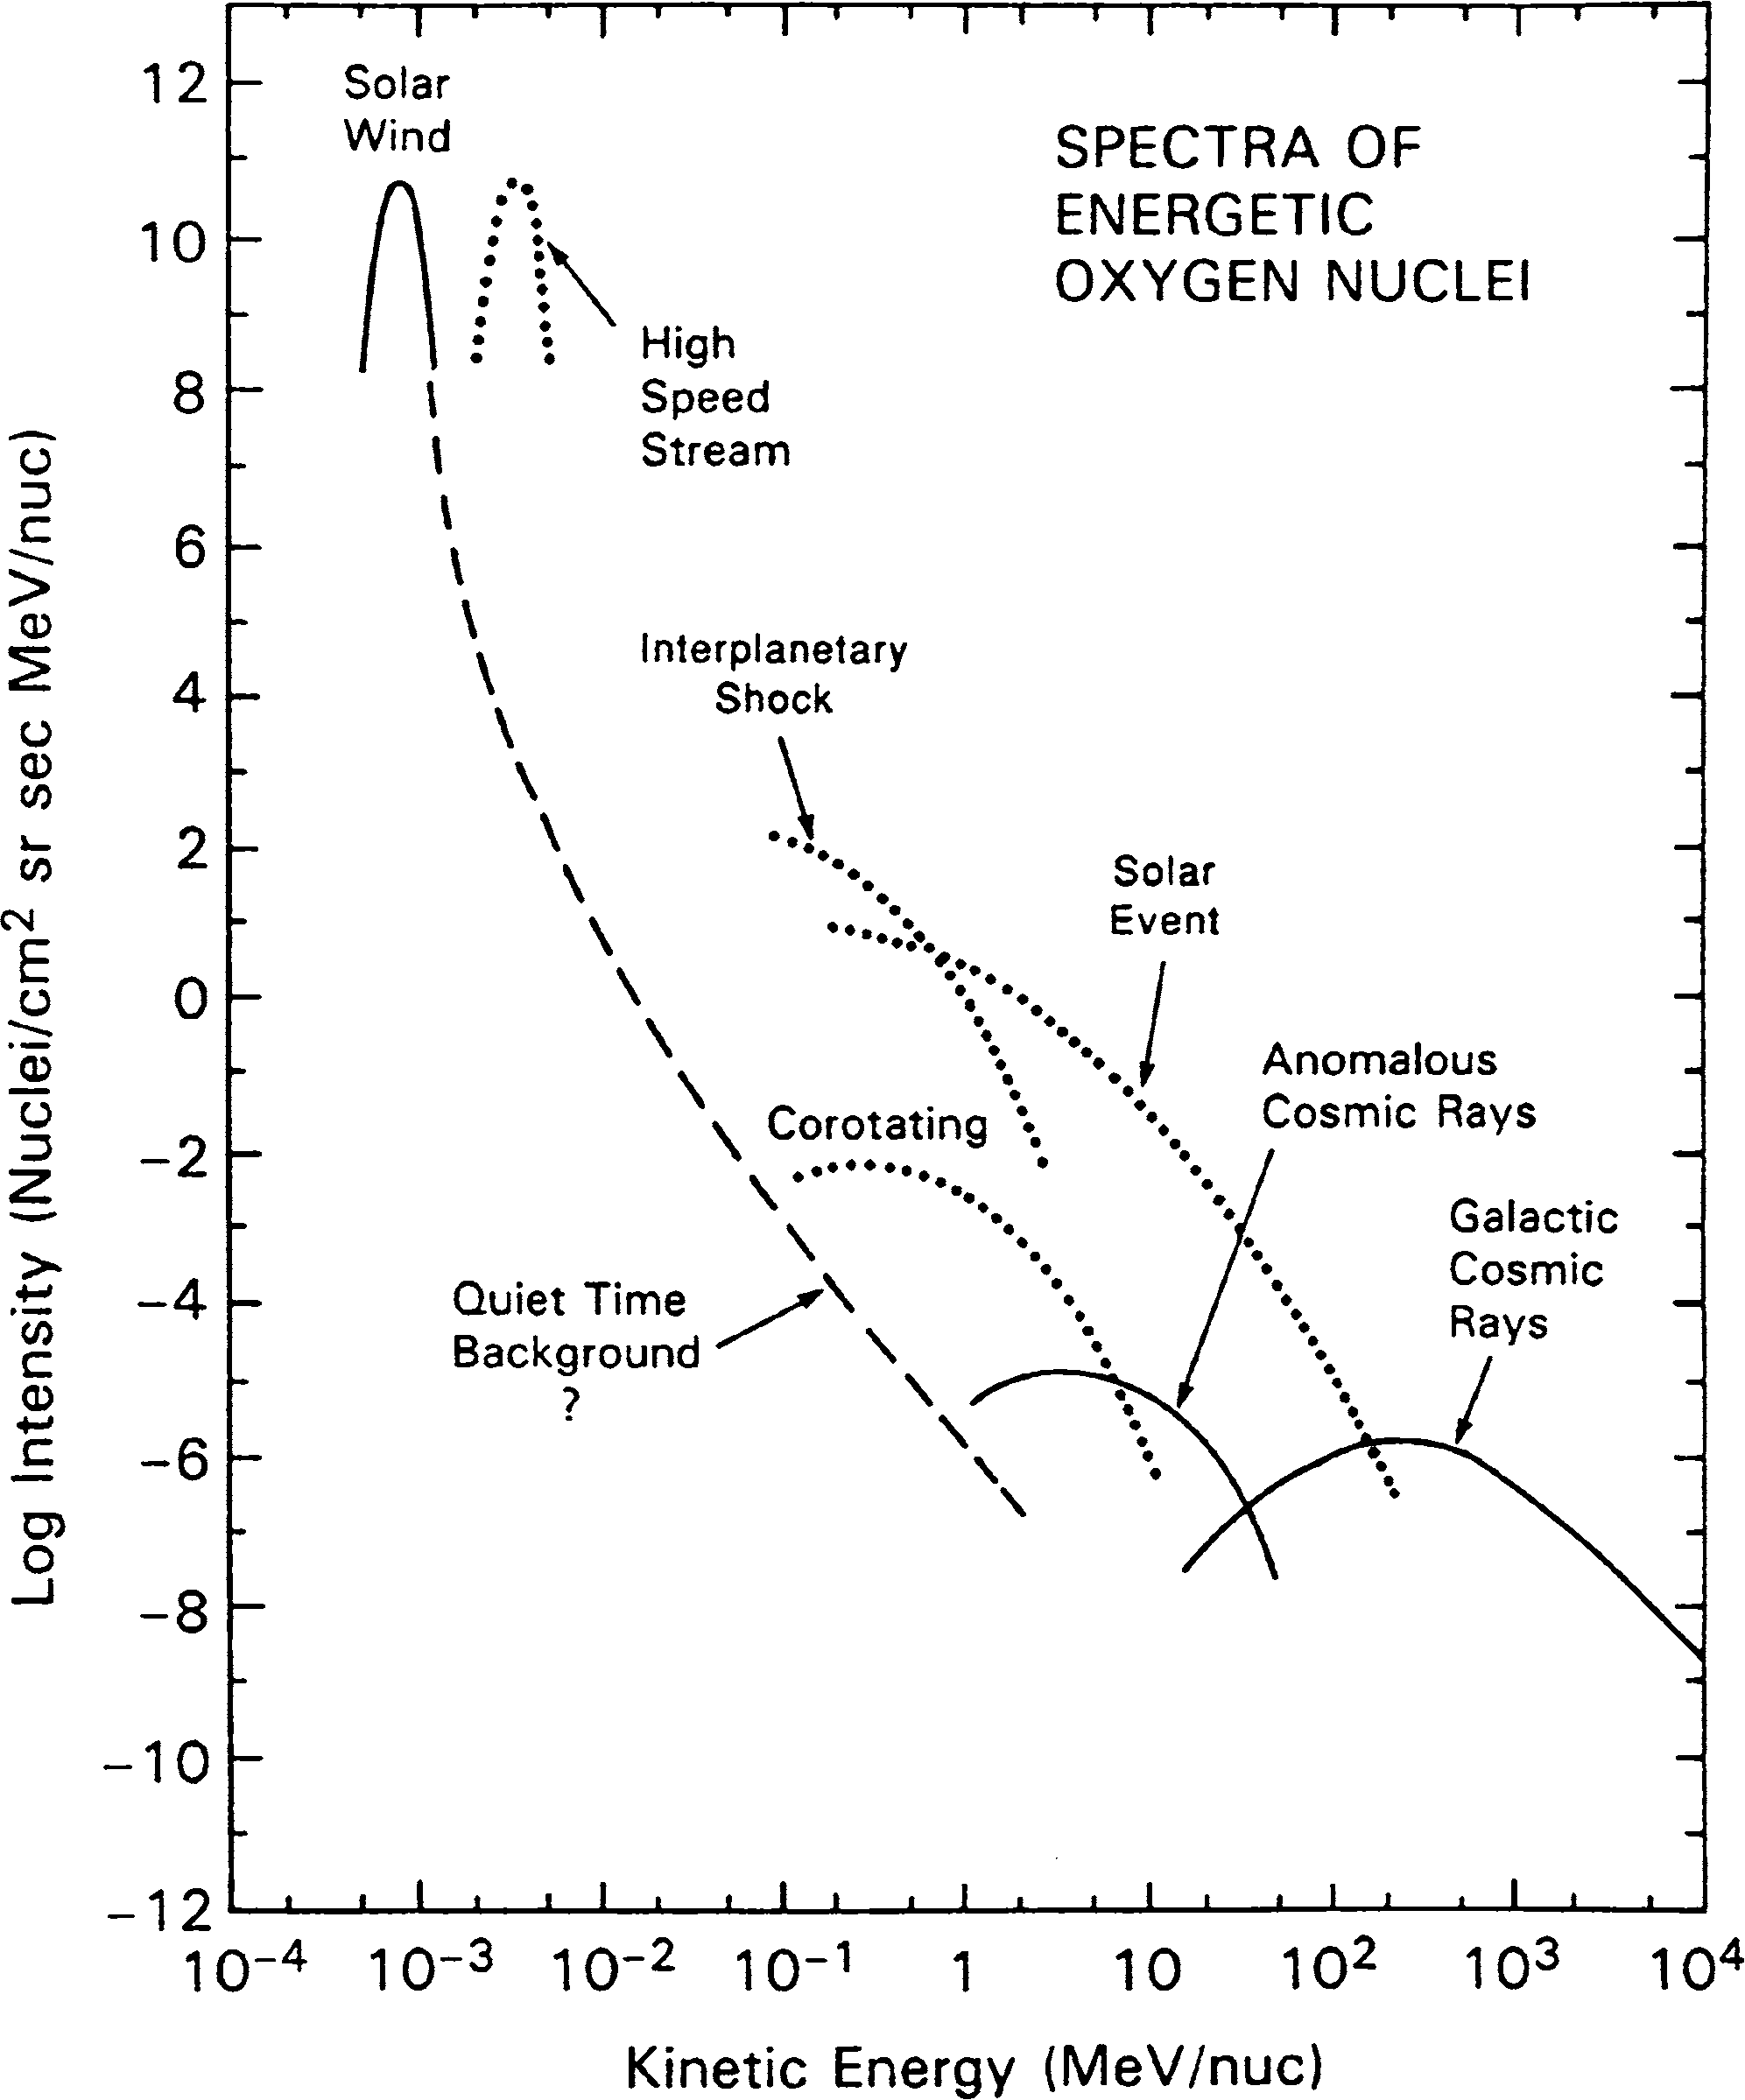
\includegraphics[width=0.6\linewidth]{images/heliospheric_energy_spectrum}
    \caption[Spectra of oxygen ions in the near-Earth interplanetary space]{Typical spectra of oxygen ions in the near-Earth interplanetary space, showing the contributions of different populations. Other particle species show similarly shaped spectra when plotted as a function of energy per nucleon (adapted from \url{http://helios.gsfc.nasa.gov/ace/gallery.html}, based on \cite{Mewaldt-2001}).}
    \label{fig:heliospheric_energy_spectrum}
\end{figure}
